\chapter{连通性}


\vspace{-1 em}
\section{连通空间}

\vspace{-1 em}
\begin{definition}[连通空间]
    设$X$是一个拓扑空间.如果存在非空、不相交的开集 $U$ 和 $V$，使得 $U \cup V = X$，则称$X$是\textbf{不连通的}，$\{U, V\}$ 是$X$的一个\textbf{分割}.否则，称$X$是\textbf{连通的}.
\end{definition}

\begin{instance}
    $\mathbb{R}_{fc}$ 是连通的.
    \begin{proof}
        假设$\{U,V\}$是$\mb{R}_{fc}$的一个分割，则$U\cap V=\varnothing,U\cup V=\mb{R}_{fc},U,V$均为开集.\par
        取$U=\mb{R}-\{a_1,a_2,\cdots,a_n\},V=\mb{R}-\{b_1,b_2,\cdots,b_m\}$，因此$U\cap V=\mb{R}-\{a_1,\cdots,a_n,b_1,\cdots,b_m\}$矛盾，因此$\mb{R}_{fc}$没有分割，因而连通.
    \end{proof}
\end{instance}

\begin{instance}
    $\mathbb{R}_l$ $\left(\text{基为} \left\{[a,b) \mid a<b\right\}\right)$ 是不连通的. \par
    取开集$U=(-\infty,0)=\bigcup_{n\in\mb{Z_+}}[-n,0)$和开集$V=[o,+\infty]=\bigcup_{n\in\mb{Z}_+}[0,n)$即可.
\end{instance}

\begin{proposition}
    $X$是不连通的 $\iff$ 存在$X$的一个非空、既开又闭的真子集.
\end{proposition}

\begin{instance}
    $\mathbb{E}^1$ 是连通的.
    \begin{proof}
        假设不然，则存在 $\mathbb{E}^1$ 的一个非空、既开又闭的真子集 $A$.\par
        假设 $b \notin A$ 且 $(b, +\infty) \cap A \neq \varnothing$.\par
        令 $d = \inf\{a \in A \mid a > b\}$.因为 $A$ 在 $\mathbb{E}^1$ 中是闭的，所以 $d \in A$.
        因此 $d > b$，且 $[b, d) \cap A = \varnothing$.\par
        这意味着 $d$ 不在 $A$ 的内部，所以 $A$ 不是开集.矛盾！
    \end{proof}
\end{instance}

\begin{definition}[连通子集]
    设$X$是拓扑空间，$A \subset X$.如果$A$在子空间拓扑中是连通的，则称$A$在$X$中是\textbf{连通的}（或$A$是$X$中的一个\textbf{连通子集}）.
\end{definition}

\begin{instance}
    $(-2, -1) \cup (1, 2) \subset \mathbb{E}^1$ 是不连通的.
\end{instance}

\begin{lemma}
    设$X$是一个拓扑空间，$A \subset X$.则$A$在$X$中是不连通的 $\iff$ 存在$X$中的开集 $U$ 和 $V$，使得 $U \cap A \neq \varnothing$, $V \cap A \neq \varnothing$, $U \cup V \supset A$，且 $(U \cap A) \cap (V \cap A) = \varnothing$.
    这样的 $\{U, V\}$ 称为$A$在$X$中的一个\textbf{分割}.
\end{lemma}
\begin{figure}[h]
    \centering
    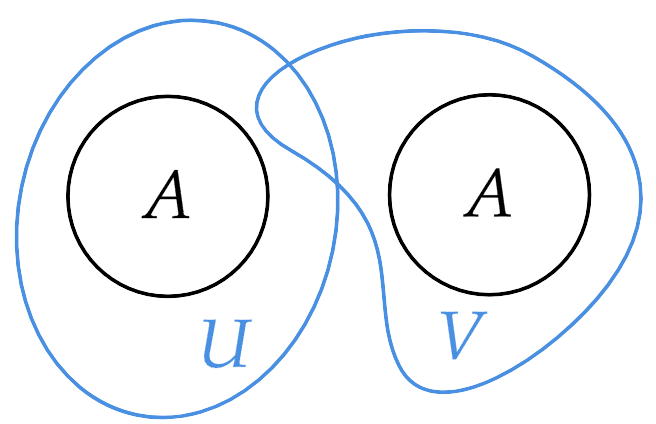
\includegraphics[width=0.3\textwidth]{fig/7.1.png}
    \captionof{figure}{}
\end{figure}


\begin{proposition}
    连通空间的连续像是连通的.即若 $f: X \to Y$ 是连续函数且 $X$ 是连通空间，则 $f(X)$ 在 $Y$ 中是连通的.
\end{proposition}
\begin{proof}
    假设不然，则存在 $f(X)$ 在 $Y$ 中的一个分割 $\{U, V\}$，即 $U$ 和 $V$ 都是开集，$U \cap f(X) \neq \varnothing$, $V \cap f(X) \neq \varnothing$, $U \cup V \supset f(X)$，且 $U \cap V \cap f(X) = \varnothing$.\par
    因为 $U \cap f(X) \neq \varnothing$ 且 $V \cap f(X) \neq \varnothing$，所以 $f^{-1}(U)$ 和 $f^{-1}(V)$ 在 $X$ 中都是非空开集.\par
    因为 $U \cap V \cap f(X) = \varnothing$，所以 $f^{-1}(U) \cap f^{-1}(V) = f^{-1}(U \cap V) = \varnothing$.\par
    因为 $f(X) \subset U \cup V$，所以 $f^{-1}(U) \cup f^{-1}(V) = X$.\par
    因此$\{f^{-1}(U),f^{-2}(V)\}$是$X$的一个分割，所以 $X$ 是不连通的.矛盾！
\end{proof}

\begin{theorem}
    设 $X_1 \cong X_2$.$X_1$ 是连通的 $\iff X_2$ 是连通的.
\end{theorem}
这个定理表示连通性是拓扑性质.

\begin{instance}
    $\mathbb{E}^1 \not\cong \mathbb{R}_l$.
\end{instance}

\begin{instance}
    $A \subset \mathbb{E}^1$，$A$ 是连通的 $\iff A$ 是一个区间.
\end{instance}
\begin{proof}
    “$\Rightarrow$” 如果 $A$ 不是一个区间，那么存在 $x$，使得 $x \notin A$，$A \cap (-\infty, x) \neq \varnothing$，$A \cap (x, +\infty) \neq \varnothing$.\par
    因此 $\{(-\infty, x), (x, +\infty)\}$ 是 $A$ 在 $\mathbb{E}^1$ 中的一个分割.矛盾！ \par
    “$\Leftarrow$” $(a, b), (a, +\infty), (-\infty, b)$ 都与 $\mathbb{E}^1$ 同胚，因此都是连通的.\par
    $[a, b]$ 是连通的，考虑函数 $f: \mathbb{E}^1 \to \mathbb{E}^1$，$x \mapsto \begin{cases} a, & x<a \\ x, & a \leq x \leq b \\ b, & x>b \end{cases}$.它是连续的，因此其像 $[a,b]$ 是连通的.\par
    $[a,+\infty)$是连通的，考虑函数 $f: \mathbb{E}^1 \to \mathbb{E}^1$，$x \mapsto \begin{cases}
        x , x\geq a\\
        2a-x,x\leq a
    \end{cases}$.它是连续的，因此其像 $[a,+\infty)$ 是连通的.\par
    因为$[a,b) \cong (a,b] \cong (-\infty,b] \cong [a, +\infty) $，$[a,b),(a,b],(-\infty,b]$是连通的
\end{proof}

\begin{theorem}[介值定理]
    设$X$是一个连通拓扑空间，$f: X \to \mathbb{E}^1$ 是连续的，$x_0, x_1 \in X$ 且 $f(x_0) < f(x_1)$.那么对于任意 $y \in [f(x_0), f(x_1)]$，都存在 $x \in X$，使得 $f(x) = y$.
\end{theorem}



\begin{lemma}
    设$X$是一个拓扑空间，$A\subset X$，$\{U,V\}$是$X$的一个分割，则要么$A\subset U$，要么$A\subset V$.
\end{lemma}
\begin{proof}
    如若不然，则$A\cap U \neq \varnothing,A\cap V \neq \varnothing$，因此$\{U,V\}$是$A$在$X$中的一个分割，所以$A$是不连通的.矛盾！
\end{proof}